\documentclass {article}

\usepackage{color}
\usepackage{amsmath}
\usepackage[margin=0.75in]{geometry}
\usepackage{graphicx}
\usepackage{chngcntr}
\usepackage{listings}
\usepackage{pdfpages}

\definecolor{Brown}{cmyk}{0,0.81,1,0.60}
\definecolor{OliveGreen}{cmyk}{0.64,0,0.95,0.40}
\definecolor{CadetBlue}{cmyk}{0.62,0.57,0.23,0}
\lstset{language=R,frame=ltrb,framesep=5pt,basicstyle=\normalsize,
 	keywordstyle=\ttfamily\color{OliveGreen},
	identifierstyle=\ttfamily\color{CadetBlue}\bfseries,
	commentstyle=\color{Brown},
	stringstyle=\ttfamily,
	showstringspaces=true}
	
\counterwithin{figure}{section}
\setcounter{secnumdepth}{5}

\begin{titlepage}

\title{\huge{\textbf{Sprint 3: LaTex Samurai}}}
\vfill
\date{April 24, 2014}
\author{\Large{Julian Brackins, Jon Dixon, Hafiza Farzami}}
\end{titlepage}

\begin{document}
	\maketitle
	\pagenumbering{gobble}
	\newpage
	\pagenumbering{roman}
	\tableofcontents
	\newpage
	\listoffigures
	\newpage
	
	\addcontentsline{toc}{section}{\LARGE{\color{blue}Mission}}
	\section*{\LARGE{\color{blue}Mission}}
		The mission statement for this project was to create a testing
		 software to test C++ source files submitted by students. The
		 testing software will automatically generate any test cases needed
		 by the user to test the source files. Each C++ source file will
		 end up with its own log file, detailing how the student performed.
		 Example statistics for a log file include: code coverage,
		 performance, and a grade percentage.\\\\The program will search
		 through all subdirectories for C++ source files to compile and run.
		 When all files have been run, a master log file is outputted in the
		 directory the test suite was ran from. This log file will only
		 contain the percent grades for each C++ file. \\\\The suite is able
		 to test programs with looping menus, and the suite itself implements
		 a looping menu.\\\\\textit{Overall, we believe that by providing a robust
		 testing suite for simple CSC150 programs, professors and TA's will
		 find that they have more time to focus on teaching, rather than the
		 tedious task of grading.}
		 
	\newpage
	
	\addcontentsline{toc}{section}{\LARGE{\color{blue}Document Preparation and Updates}}
	\section*{\LARGE{\color{blue}Document Preparation and Updates}}
		Current Version [1.2.0]\\
		
		{\noindent
		\textit{Prepared By:}\\
		\textit{Jonathan Dixon}\\
		}
		
		\vfill
		\textit{\color{blue}Revision History}\\
		\begin{tabular}{|c|c|c|c|}
		\hline 
		\textbf{Date} & \textbf{Author} & \textbf{Version} & \textbf{Comments} \\ 
		\hline 
		2/17/14 & Hafiza Farzami & 1.0.0 & Initial Version \\ 
		\hline 
		3/23/14 & Hafiza Farzami & 1.1.0 & Edited version for Sprint 2 \\ 
		\hline 
		4/24/14 & Jonathan Dixon & 1.2.0 & Added Sprint 3 functionality \\ 
		\hline 
		\end{tabular} 
		
	\newpage
	
	\pagenumbering{arabic}

		
	\section{\LARGE{\color{blue}Overview and Concept of Operations}}
	
		This report will cover the project overview, user stories, backlog,
		 design and implementation, development, environment, deployment, and 
		 documentation for the testing project.\\\\
		 
		 \subsection{\Large{\color{blue}Scope}}
		 	This document covers the details of the project including its
		 	 functionality, tools used, and the process that led to a
		 	 valid solution that fulfills all of the requirements.
		 	 
		 \subsection{\Large{\color{blue}Purpose}}
		 	The purpose of this program is to run entire directories of
		 	 .cpp files with given test files, and grade them. There are
		 	 certain tests that are labeled as critical tests; if a .cpp
		 	 file does not pass one of the critical tests, there is no grade
		 	 assigned. Otherwise the percentage of tests passed is
		 	 calculated for each .cpp file.
		 	 
		 	\subsubsection{\large{\color{cyan}Traversing Subdirectories}}
		 		\paragraph{Functionality}
		 			Traversing subdirectories is one of the main components of
		 			 this system. The testing suite will seek out all
		 			 subdirectories below its beginning working directory. From
		 			 that point, it will compile and run any .cpp file with a
		 			 name that matches the name of its directory. For example:
		 			 \begin{equation*}
		 			 	/home/Documents/CSC150/Prog1/JohnDoe/JohnDoe.cpp
		 			 \end{equation*}
		 			 will be compiled and tested, whereas:
		 			 \begin{equation*}
		 			 	/home/Documents/CSC150/Prog2/submits/JohnDoe.cpp
		 			 \end{equation*}
		 			 will not be compiled.
		 		 
		 		 \paragraph{Convenience}
		 		 	The convenience of this becomes clear when one realizes that
		 		 	 an entire directory of students' files may be tested from a
		 		 	 single program execution, from one location. This will
		 		 	 encompass all subdirectories, giving the potential for a
		 		 	 professor or TA to grade more than one project at one time.
		 		 
			\subsubsection{\large{\color{cyan}Generating Test Cases}}
				The testing suite is a fully functioning test case generator.
				 If the user chooses, it will generate .tst files containing
				 ints, doubles, or random strings. These tests are then
				 stored in the \textit{/tests} subdirectory, which is on the
				 same level as the folders containing students' .cpp files.
				 Since the suite also keeps track of code coverage, if a user
				 has reviewed a student's .log file and found that coverage
				 was not 100 percent, the user may wish to generate
				 additional test cases.		 		 
		 		 
		 	\subsubsection{\large{\color{cyan}Compiling and Running .cpp Files}}
		 		This software will use Linux system calls and the GNU
		 		 Common Compiler to build all .cpp files to be tested.
		 		 Since these programs will expect all input from the
		 		 command line, we must redirect input from the .tst files.
		 		 The .cpp to be tested will be ran on each of the .tst
		 		 files.
		 		 
		 \subsection{\Large{\color{blue}Systems Goals}}
		 	The goal of the system is to make grading a less tedious
		 	 task. This product grades an entire directory of .cpp files
		 	 by simply executing from the root directory! The product is
		 	 built to test the .cpp file with all of the given or
		 	 generated .txt test files in the current directory, and
		 	 compare the results to the corresponding .ans files. The
		 	 product also has the functionality to test any menu-driven
		 	 .cpp files that may use a simple text-based menu.
		 		 
		 \subsection{\Large{\color{blue}System Overview and Diagram}}
		 	This section contains a flow diagram detailing an overview
		 	 of the entire system.\\\\
		 	\begin{figure}[h!]
		 		\centering
				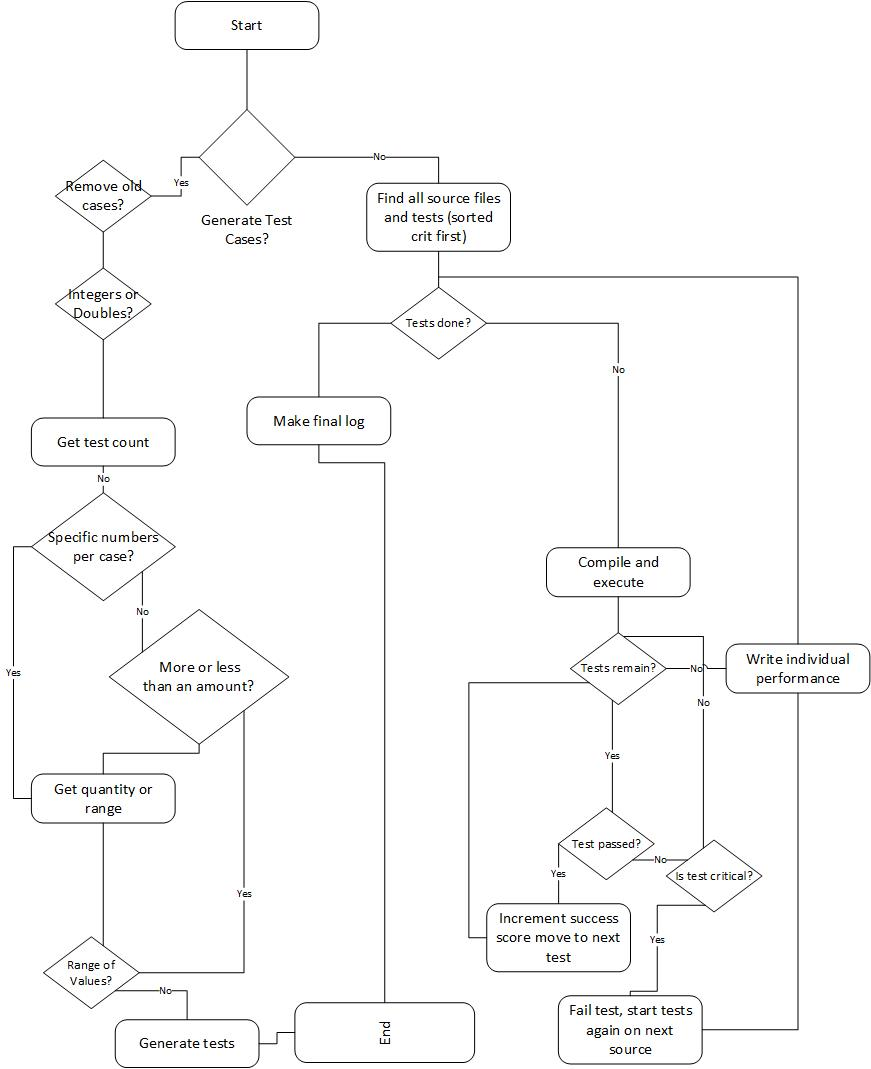
\includegraphics[width=0.7\linewidth]{diagram.jpg}
				\caption{Flow Diagram}
				\label{fig:Flow_Diagram}
			\end{figure}
		 		
		 \newpage
		 		
	\section{\LARGE{\color{blue}Project Overview}}
		This section will contain an overview of the people and processes
		 used to reach the completion of our product.
		 	 
		 	\subsection{\Large{\color{blue}Team Members and Roles}}
		 	 	\begin{enumerate}
		 	 		\item Julian Brackins - Product Owner
		 	 		\item Jon Dixon - Scrum Master
		 	 		\item Hafiza Farzami - Technical Lead
		 	 	\end{enumerate}
		 	 	
		 	\subsection{\Large{\color{blue}Project Management Approach}}
		 		We used an agile approach to this project. This involves frequent
		 	 	 meetings called \textit{scrum meetings}, which are orchestrated
		 	 	 by the scrum master. The product owner was in charge of getting
		 	 	 in touch with Dr. Logar (the customer) to present any questions
		 	 	 or other concerns. The technical lead took point on the coding,
		 	 	 but was supported by the other roles. The project was split into
		 	 	 small, manageable chunks using trello as a way to keep track of
		 	 	 all of the tasks visually.
		 	 	 
			\subsection{\Large{\color{blue}Phase Overview}}
				Since every large task has been broken up into smaller pieces, we
				 essentially keep track of progress by noting when each small part
				 is complete, and then moving on to the next step for that task.
				 When all steps for a task have been completed, the next task will
				 be undertaken using the same principles for dividing the work.
				 This process continues until all tasks, and the project, have
				 been completed.
		 	 
		 \newpage
		 
	\section{\LARGE{\color{blue}User Stories, Backlog, and Requirements}}
		\subsection{\Large{\color{blue}Overview}}
	 		This section will cover all of the user requirements for the product,
	 		 and how we have laid out a framework for the completion of the
	 		 project. We will touch on stakeholder information, the business need
	 		 for our product, requirements and design constraints, and user
	 		 stories.
	 		 
	 		\subsubsection{\large{\color{cyan}Scope}}
	 			The scope of this product is not incredibly broad. The system is
	 			 highly specialized to test CSC 150 programs that will take input
	 			 from the command line, and output results to the command line.
	 			 We have implemented code to test programs with menus. It would be
	 			 possible to generalize this to handle programs with file input
	 			 and output, but it would take some time to implement.
		 		
	 		\subsubsection{\large{\color{cyan}Purpose of the System}}
	 			The purpose of the system is to allow a professor or TA to grade
	 			 entire directories of CSC 150 programs, including programs that
	 			 implement text-based menu loops. The system will also keep track
	 			 of the code coverage and performance of all programs tested.
	 			 
	 	\subsection{\Large{\color{blue}Stakeholder Information}}
	 		This section will provide all basic information on the stakeholders
	 		 involved in this project.
	 		
	 		\subsubsection{\large{\color{cyan}Customer or End User (Product Owner}}
	 			For sprint 3, Julian Brackins was the product owner. He worked with
	 			 Dr. Logar to gather requirements, and relay them to the rest of
	 			 the team.
	 		
	 		\subsubsection{\large{\color{cyan}Management or Instructor (Scrum Master)}}
	 			Jon Dixon was the scrum master for sprint 3. The scrum master
	 			 is responsible for breaking the main project up into larger tasks
	 			 and keeping in touch with the product owner and technical lead
	 			 to make sure the work is being completed in a timely manner.
	 			 
	 		\subsubsection{\large{\color{cyan}Developers - Testers}}
	 			Hafiza Farzami was the technical lead for sprint 3. She kept in
	 			 touch with the scrum master and product owner to make sure all
	 			 tasks were being completed in a timely manner. Testing was done
	 			 by all team members, since the developers and testers are the
	 			 same group.
	 			 
	 	\subsection{\Large{\color{blue}Business Need}}
	 		The business need for this project is clear. Since the purpose is to
	 		 save time for professors and TA's, these people can spend their time
	 		 focusing on more important matters such as developing a more robust
	 		 curriculum, and devoting more time to the students, ensuring a higher
	 		 quality education.
	 		 
	 	\subsection{\Large{\color{blue}Requirements and Design Constraints}}
	 		This section outlines the what a user will need to be able to run the
	 		 program. This includes operating system, additional programs, etc...
	 		 
	 		 \subsubsection{\large{\color{cyan}System Requirements}}
	 		 	The program is designed to run on Linux machines, that are capable
	 		 	 of running both gcov and gprof. It uses the GNU Compiler
	 		 	 Collection.
	 		 	 
	 		 \subsubsection{\large{\color{cyan}Network Requirements}}
	 		 	This program requires no active internet connection to function
	 		 	 properly.
	 		 	 
	 		 \subsubsection{\large{\color{cyan}Development Environment Requirements}}
	 		 	This program requires no special development environment.
	 		 	
	 		 \subsubsection{\large{\color{cyan}Project Management Methodology}}
	 		 	We used an agile method to project management. The process is
	 		 	 described below.
	 		 	\begin{enumerate}
	 		 		\item Product Owner meets with Dr. Logar.
	 		 		\item Product Owner meets with Scrum Master and Technical Lead
	 		 			\begin{enumerate}
	 		 				\item Break large projects into smaller tasks.
	 		 				\item Assign these tasks to team members
	 		 				\item Create cards on the Trello board to represent
	 		 				 the tasks.
	 		 			\end{enumerate}
	 		 		\item Team members work on their tasks, updating the Trello
	 		 		 board as necessary.
	 		 		\item Frequent ten-minute scrum meetings to keep track of
	 		 		 progress.
	 		 		\item Repeat entire process for each sprint.
	 		 	\end{enumerate}
	 		 	
	 	\subsection{\Large{\color{blue}User Stories}}
	 		This section will contain the complete collection of user stories for
	 		 sprints 1, 2, and 3. It will also contain details on how we broke
	 		 these stories down into tasks that we needed to implement in our
	 		 product.
	 		 
	 		\subsubsection{\large{\color{cyan}User Story \#1}}
	 			As a user, I would like a program to be able to grade a specified
	 			 directory of CSC 150 programs. I would like this program to be
	 			 able to generate test cases, detect programs with infinite loops,
	 			 and record performance of each program.
	 			 
	 			\paragraph{\textbf{User Story Breakdown \#1}}
	 				\ \\ \ \\The program needs to be able to "crawl" through directories to
	 				 find test cases, answer cases, and and .cpp files that have been
	 				 submitted by students. The program should be able to grade an
	 				 entire directory by running it only once.		 				 
	 				 
	 				\begin{figure}[h!]
	 					\centering
							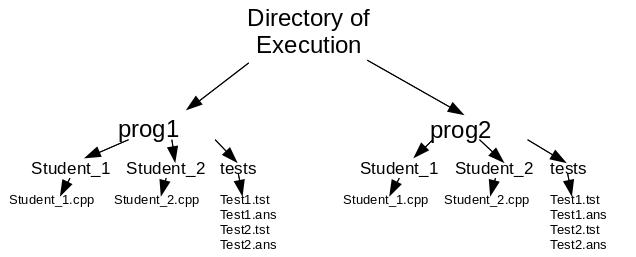
\includegraphics[width=0.7\linewidth]{Figure1.jpg}
							\caption{Directory Structure}
							\label{fig:Directory_Structure}
					\end{figure}
					
	 		\subsubsection{\large{\color{cyan}User Story \#2}}
	 			I would like to be able to view each student's performance for all test
	 			 cases, code coverage of all test cases, and code performance for all test
	 			 cases.
	 			\paragraph{\textbf{User Story Breakdown \#2}}
					\ \\ \ \\For each student, a log file will be produced. This log file will
					 contain the following information:
					 	\begin{itemize}
				 		\item Pass or failure for each test case
				 		\item Gcov statistics for code coverage
				 		\item Gprof statistics for code performance
				 	\end{itemize}
					 	
					Each of these log files will have the following structure:\\\\
					
					\centering
						\indent	passed {\tt or} failed:	\indent case$_{\text{1}}$.tst \\*
						\indent	passed {\tt or} failed:	\indent case$_{\text{2}}$.tst \\*
						\indent \indent \indent \indent \indent \indent	.				 \\*
						\indent \indent \indent \indent \indent \indent	.				 \\*
						\indent \indent \indent \indent \indent \indent	.				 \\*
						\indent	passed {\tt or} failed:	\indent case$_{\text{n}}$.tst \\*
						\indent Lines Executed: xxx.xx\% out of x\\*
						\indent \textless GPROF STATISTICS FOR EACH FUNCTION\textgreater
						
					\raggedright
						
						
	 		\subsubsection{\large{\color{cyan}User Story \#3}}
	 			I would like there to be a common summary log file containing the grades
	 			 (as percentages) of all students, which students failed, and average class
	 			 statistics, such as how many students passed.
	 			 
	 			\paragraph{\textbf{User Story Breakdown \#3}}
	 				\ \\ \ \\The specified log file will be located in the subdirectory the user
	 				 specified as the test directory and will contain the following structure:\\ \ 							 \\
	 				
	 				\centering
						\indent	Student$_{\text{1}}$.cpp:	\indent Percent grade \\*
						\indent	Student$_{\text{2}}$.cpp:	\indent Percent grade \\*
						\indent \indent \indent \indent \indent \indent	.				 \\*
						\indent \indent \indent \indent \indent \indent	.				 \\*
						\indent \indent \indent \indent \indent \indent	.				 \\*
						\indent	Student$_{\text{n}}$.cpp:	\indent Percent grade
						
					\raggedright
					
					
	 		\subsubsection{\large{\color{cyan}User Story \#4}}
	 			I would like to be able to generate test cases to run the programs on.
	 			
	 			\paragraph{\textbf{User Story Breakdown \#3}}
	 				\ \\ \ \\Upon execution of the program, the user will be prompted to see if
	 				he or she would like to generate test cases. Test cases may be of three types:
	 				
	 				\begin{itemize}
	 					\item Floating point numbers
	 					\item Integers
	 					\item Strings
	 				\end{itemize}
	 				
	 				No matter which option the user chooses, they will be prompted for the number
	 				 of test cases to generate, number of items per test case,
	 				 the minimum and maximum random number bounds
	 				 (Floats and Ints only), and string length (strings only). If they have chosen
	 				 string generation, the strings will be composed of lowercase alphanumeric
	 				 characters, and the numbers 0-9.
	 				 
	\newpage
	 	
	\section{\LARGE{\color{blue}Design and Implementation}}
		This section is used to describe the design details for each of the major components 
		 in the system.
		 
		\subsection{\Large{\color{blue}Finding Test Cases (find tsts function)}}
			\subsubsection{\large{\color{cyan}Technologies Used}}
				\begin{itemize}
   					\item popen
    				\item GNU find
    				\item C++ vectors
				\end{itemize}
				
			\subsubsection{\large{\color{cyan}Component Overview}}
				This component uses the GNU find program to recursively find all filenames of the
				 form *.tst. This will also look in all subdirectories. Popen is then used to
				 capture all of the output, which is then places in a vector that will store all
				 of the test case filenames.
				 
			\subsubsection{\large{\color{cyan}Phase Overview}}
				This component was initially developed for Sprint 1, and has been an integral part
				 in all subsequent sprints, since .tst files have always needed to be identified.
				 
			\subsubsection{\large{\color{cyan}Design Details}}
				One issue when designing this component was that there was a character at the end
				 of all filenames that needed to be removed. Luckily, we found that the we were
				 able to remove it with the simple block of code below.
\begin{lstlisting}
//removing that frustrating invisible character at the end of the strings
for(int i=0;i<tstfilelist.size();i++)
{
	tstfilelist.at(i).replace(tstfilelist.at(i).end()-1,
	tstfilelist.at(i).end(),"");
}
\end{lstlisting} 
				 
				 
		\subsection{\Large{\color{blue}Running the Student Programs (run tests function)}}
			\subsubsection{\large{\color{cyan}Technologies Used}}
				 \begin{itemize}
   					\item C++ vectors
    				\item gcov
    				\item gprof
				\end{itemize}
				
			\subsubsection{\large{\color{cyan}Component Overview}}
				This function is used to compile and run the .cpp files using the .tst files as
				 input. Initially, the component could only check one .cpp file, but it has since
				 been extended to use a vector of filenames to compile and run multiple files.
				 It will compile each .cpp file with flags for gcov and gprof. Gcov is also
				 executed within this component.
				 
			\subsubsection{\large{\color{cyan}Phase Overview}}
				This component was initially implemented for Sprint 1, but it only would work for
				 a single .cpp file. For Sprint 2, it was extended to function for all .cpp files
				 in a directory, and gcov and gprof functionality was added.
				 
			\subsubsection{\large{\color{cyan}Design Details}}
				Before any of the programs may be run, we must first check to see if they have
				 been compiled. If the program has already been compiled, there is no need to
				 compile it again. If a program has not been compiled, we will compile it with
				 the following bit of code:
\begin{lstlisting}
string prog_cpp = prog;
string progname = prog_cpp.substr(0,prog_cpp.find("."))
string progcomp = "g++ -pg -fprofile-arcs -ftest-coverage -o "+progname+" "+prog_cpp;

ifstream fileExists(progname.c_str());
if (!fileExists)
{
    fileExists.close();
    
    //compile program to be tested
    system(progcomp.c_str());
}
else
{
	//close input check
    fileExists.close();
}
\end{lstlisting} 

				Prog is the full file path to the .cpp file, including the filename.\\ \ \\It is
				 also important to note that this function will also call the proper function to
				 fork a child process containing the student's test file. This is accomplished 
				 with a simple calls to fork and exec. A progress bar is also created to display
				 how close a program is to reaching the specified time for an "infinite loop"
				 case. If any process should reach that time limit, it will be killed, and marked
				 as a failure.\\ \ \\The function is also responsible for gcov. Each time after
				 execution, the program will update it's .covs file, which is the extension for
				 redirected gcov output. This will accurately represent the code coverage, since
				 the .gcno file containing the gcov notes has not been deleted or modified in
				 this time. \\ \ \\The function will then check the result of the execution
				 against the .ans file that corresponds to the current .tst file. The function
				 will return 0 if the answer was correct, 1 if the answer was incorrect, or -1 if
				 the files could not be opened for comparison for any reason.
				 
		\subsection{\Large{\color{blue}Checking Student Output (files equal function)}}
			\subsubsection{\large{\color{cyan}Technologies Used}}
				 \begin{itemize}
   					\item C++ vectors
				\end{itemize}
				
			\subsubsection{\large{\color{cyan}Component Overview}}
				This component simply will take two files as input and return true or false
				 as to if they are equal or not.
				 
			\subsubsection{\large{\color{cyan}Phase Overview}}
				This component was originally developed in Sprint 1, and has been useful ever
				 since.
				 
			\subsubsection{\large{\color{cyan}Design Details}}
				This function will compare two files by reading their contents into vectors.
				 These vectors are then compared, and if they are the same length and have the
				 same contents, the files are determined to be equivalent.
				 
				 
		\subsection{\Large{\color{blue}Finding Student Code (find\_students)}}

			\subsubsection{\large{\color{cyan}Technologies  Used}}
			\begin{itemize}
				\item C++ vectors
				\item Dirent directory file descriptors
			\end{itemize}

			\subsubsection{\large{\color{cyan}Component Overview}}
				This component searches for every student source file and adds it to the list of
				 the programs to be compiled and executed

			\subsubsection{\large{\color{cyan}Phase Overview}}
				This component was designed and developed second phase as an integral part of
				 2.0.0 functionality.

			\subsubsection{\large{\color{cyan}Design Details}}
				This component is designed to recursively scan all sub-directories for any source
				 files.
				 
\begin{lstlisting}
while (entry = readdir(dir)) 
  {
    temp = entry->d_name;
    if ( temp != "." && temp != ".." )
    {
      if ( temp[temp.size() - 1] != '~' )
      {
        int length = temp.length();
        if ( (length > 4 && (temp.substr(length-4) == ".cpp")
             || temp.substr(length-2) == ".C")
             && level > 0 )
        {
          STUDENTVECTOR.push_back(directory + '/' + temp);
        }
        else if ( (length > 4 && (temp.substr(length-4) == ".cpp")
             || temp.substr(length-2) == ".C")
             && level == 0 )
        {
          if (GOLDCPP.empty())
          {
            GOLDCPP = directory + '/' + temp;
          }
        }
        else
        {
          find_students(directory + '/' + temp, level + 1);
        }
      }
    }
  }
\end{lstlisting}

		\subsection{\Large{\color{blue}Write Individual Report (writeindividualreport function)}}

			\subsubsection{\large{\color{cyan}Technologies  Used}}
				\begin{itemize}
					\item C++ vectors
				\end{itemize}

			\subsubsection{\large{\color{cyan}Component Overview}}
				This component writes an individual report regarding each test as they happen in
				 the current program's directory.

			\subsubsection{\large{\color{cyan}Phase Overview}}
				This component was designed and developed second phase as an integral part of
				 2.0.0 functionality.

			\subsubsection{\large{\color{cyan}Design Details}}
				This component will simply advise if a program has passed or failed a specific
				 test.  After a critical fail, the remaining tests will not be ran or logged.
				 It will push the result onto a vector of results for each student. This vector is
				 later used to output the student's individual log file.
				 
				 
		\subsection{\Large{\color{blue}Detecting Presentation Errors}}
			\subsubsection{\large{\color{cyan}Technologies  Used}}
				\begin{itemize}
					\item C++ string streams
				\end{itemize}
			
			\subsubsection{\large{\color{cyan}Component Overview}}
				The presentation error function compares strings, it it is a presentation error,
				 it counts it, returns zero otherwise.
				 
			\subsubsection{\large{\color{cyan}Phase Overview}}
				We implemented this feature in sprint three because it was added functionality
				 for this sprint. 
				 
			\subsubsection{\large{\color{cyan}Design Details}}
				Given the solution and the student files, this feature runs diff file command, and
				 returns the difference into a third file, 'a.out'. The code then goes through
				 the new file and compares the strings. If the descriptors have the same first and
				 last letters and are the same size, or are anagrams, they are marked as
				 presentation error. If the value that differs, rounds to the correct answer, is 
				 also marked as a presentation error. The following code demonstrates
				 how we count the errors.
				 
\begin{lstlisting}
int prezErrorCount( string file1, string file2 ) 
{
	ifstream difference( "a.out" );
	system(
		("diff -b -y -i --suppress-common-lines "
		+file1+" "+file2+" > a.out" ).c_str());
	string line;
	subs dif;
	int errors = 0;
	
	while( getline( difference, line ) )
	{
		dif = subStrings( line, '|' ); 
		istringstream desc( dif.first );
 	        istringstream val( dif.last );
		
		errors += markError( desc, val );
	}	

	difference.close();
	return errors;
}
\end{lstlisting}	


	\newpage
	
	\section{\LARGE{\color{blue}System and Unit Testing}}
		This section will detail the methods and approaches the team took with regard to both
		 system and unit testing.
		 
		\subsection{\Large{\color{blue}Overview}}
			Overall, a lot of our testing started with unit testing, and moved its way up to
			 integration testing as we went along. Since we were not provided with any example
			 student .cpp files for this sprint, we had to come up with our own files that would
			 simulate student mistakes such as infinite loops and presentation errors.
			 
		\subsection{\Large{\color{blue}Dependencies}}
			This program is written with the assumption that the file directory structure will
			 follow the structure laid out in Figure 3.1.
			 
		\subsection{\Large{\color{blue}Test Setup and Execution}}
			In sprints one and two, Dr. Logar provided us with many of the necessary testing
			 materials, such as .cpp files to test, and the directory with the expected structure.
			 In this sprint, she did not provide any additional content. We found that some of
			 the materials we needed to perform tests, such as programs with presentation errors,
			 infinite loops, or programs that sorted strings were easy to produce from either
			 code that we had already created, or from scratch. Overall, we tested the entire
			 program in small chunks before attempting to integrate into the larger system.
			 \\ \ \\For example, when developing the code for gcov, we first wrote a small,
			 menu-driven program with a few options that would simply output a line of code when
			 the option was chosen. We compiled with the gcov flags, and ran the program and gcov
			 to see the results. As expected, gcov reported that not all of the lines of code had
			 been executed. With this in mind, we ran the program again, and chose the other
			 menu options. This resulted in a gcov output that 100\% of the lines had been
			 executed. From there it was only a matter of getting all of the filenames and
			 directories correct when integrating gcov into the main algorithm. This type of
			 unit testing was the main driving force behind most of the testing of our system.
			 \\ \ \\As far as our user interface is concerned, we made sure that it would catch
			 any errors outside of the bounds of the possible input choices, or receiving input
			 that is a character instead of an integer.
			 
	\newpage
	
	\section{\LARGE{\color{blue}Development Environment}}
		This section serves the purpose of providing the user with the necessary information
		 to compile and run our test suite code on his or her machine.
		 
		\subsection{\Large{\color{blue}Development IDE and Tools}}
			In the creation of this program, we did not use any special development IDE, or tools.
			 We used mainly gedit, vim and the g++ compiler to develop and test our code. One of
			 the most useful tools we used was the Makefile that is included with our .cpp files.
			 When compiling our code we strongly suggest that the user do so by simply typing
			 "make" in the directory containing the makefile and all of the source code.
			 
		\subsection{\Large{\color{blue}Source Control}}
			We found that using git and github for source control was very useful. We did our
			 best to make frequent commits of only working software. Git allowed us to
			 collaborate easily on our project, providing an interface for merging and backups
			 of previous versions. This proved useful at one point in particular, as a merge 
			 gone wrong found us missing a sizeable portion of new code that we had just written.
			 Since github contains copies of all previous versions, we were able to recover
			 the code from before the merge removed the new code that we created.
			 
		\subsection{\Large{\color{blue}Dependencies}}
			From a user's perspective, the dependencies are low. All that is required of a user is
			 a working linux operating system with the GNU compiler collection. From a
			 development perspective, it is necessary to have a github account with access to the
			 git repo used by the development team, as well as the requirements that apply to the
			 user.
	
		\subsection{\Large{\color{blue}Build Environment}}
			The only build environment requirements are Linux and a recent version of the GNU
			 compiler collection. A makefile has been provided for convenience.
			 
		\subsection{\Large{\color{blue}Development Machine Setup}}
			A development machine simply needs access to the git repo and a clone of the git
			 repository.
	
	\newpage
	
	\section{\LARGE{\color{blue}Release - Setup - Deployment}}	
		This section will contain any specific subsection regarding specifics in releasing, setup,
		 and/or deployment of the system.	
	
		\subsection{\Large{\color{blue}Deployment Information and Dependencies}}
			\begin {itemize}
				\item Validate your linux installation has a current install of gcc (yum -install
				 gcc / apt-get install gcc / emerge install gcc  / pacman -S gcc)
				\item (Optional / Troubleshooting) validate linux headers are installed (above
				 package manager with the arguments: linux-headers-\$(uname -r))
			\end {itemize}	
			
		\subsection{\Large{\color{blue}Setup Information}}
			Simply run the makefile using the following command: "make".\\Invoke the program by
			 typing ./test. The user interface will be presented, and the user may follow the
			 on-screen directions.
			 
		\subsection{\Large{\color{blue}System Versioning Information}}
			All system version information is stored on the github including time of updates,
			 previous versions, and who authored each change.
			 
	\newpage
	
	\section{\LARGE{\color{blue}User Documentation}}
		This section will provide users with a brief overview of the features that we have
		 implemented in the final CSC150 program testing suite.	
		 
		\subsection{\Large{\color{blue}User Guide}}
		 	The test executable must be located one directory above the directories that the
		 	 program may be asked to test. The program expects to be given the name of a "golden"
		 	 .cpp file that will contain the code to create the answer cases.
		 	 
		 	\begin{figure}[h!]
				\centering
				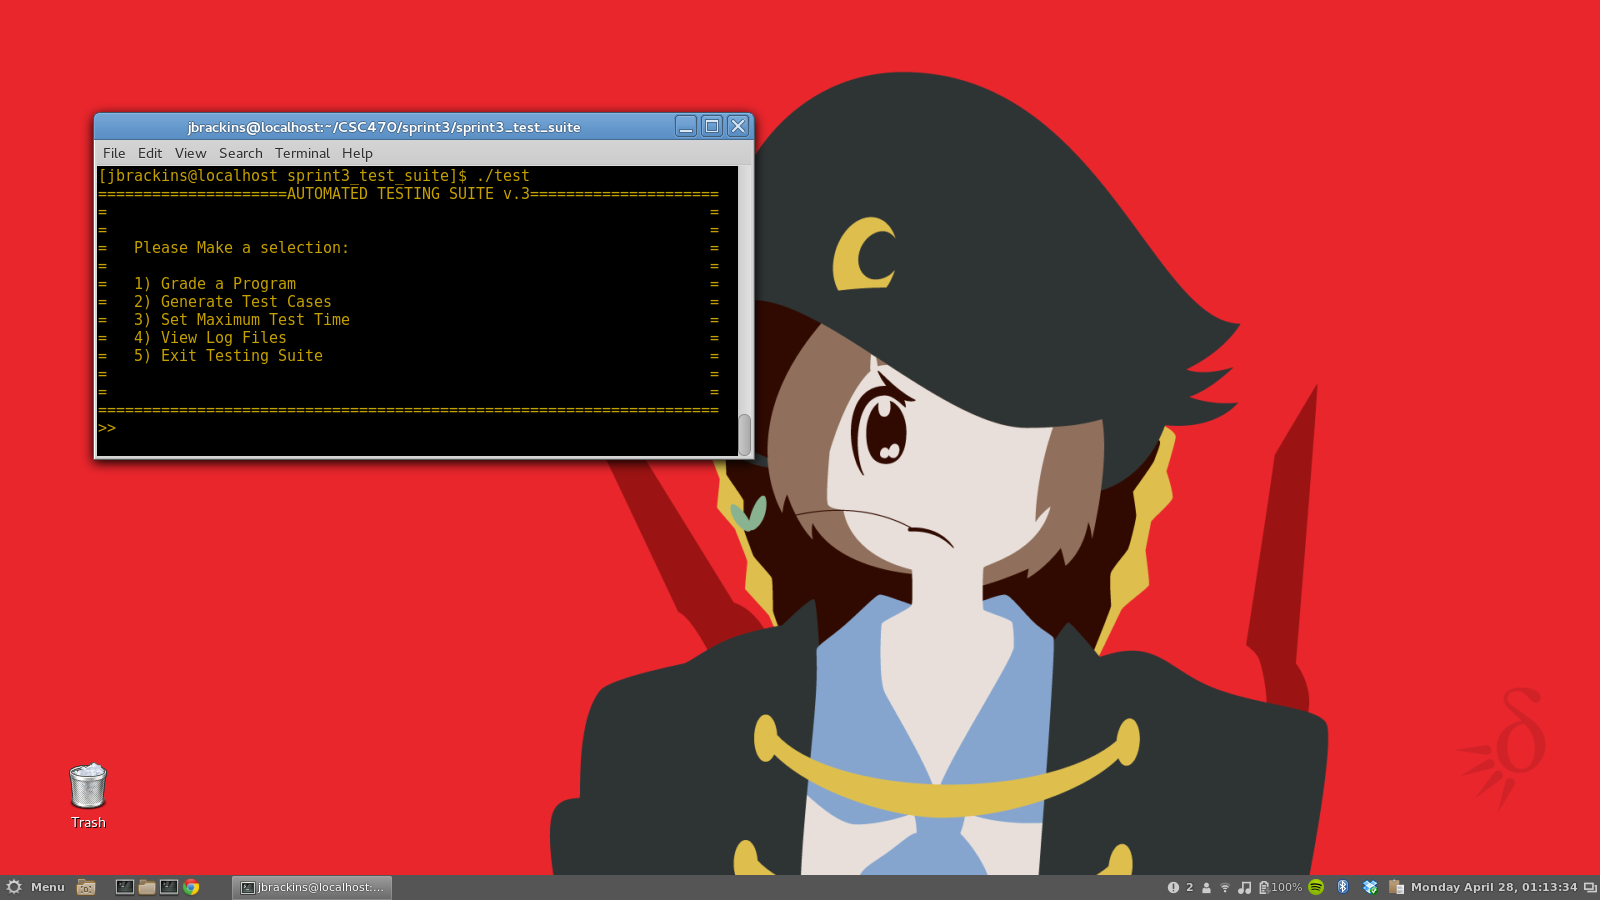
\includegraphics[width=0.6\linewidth]{mainmenu.png}
				\caption{User Interface Main Menu}
				\label{fig:main_Menu}
			\end{figure}
			
			The interface will involve typing a numerical value that is associated with a menu
			 choice, typing a directory name, or answering questions about test case generation.
			 The main menu of the user interface provides the user with a number of options related
			 to the grading and reviewing of student .cpp files.
			
					 	 
		 	\begin{figure}[h!]
				\centering
				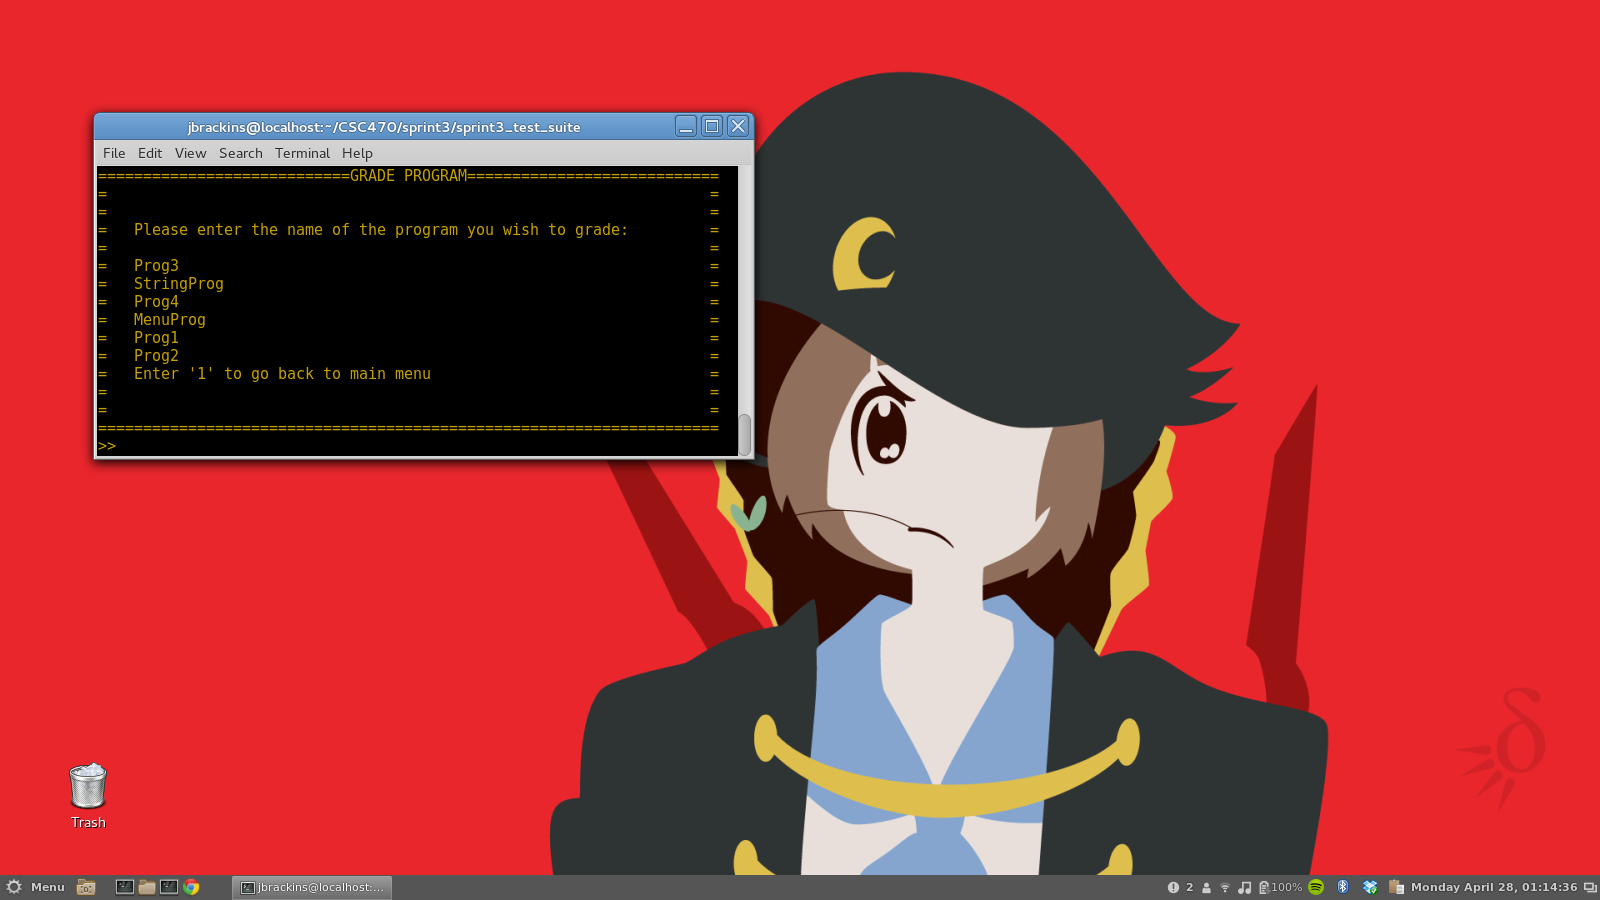
\includegraphics[width=0.6\linewidth]{gradeprog.png}
				\caption{Selecting a Program to Grade}
				\label{fig:grading_Program}
			\end{figure} 
			
			In this example, the user will type the directory name of the program they would like
			 to grade. After doing so, they will be prompted for the name of the "golden" .cpp 
			 file. 
			 
		 	\begin{figure}[h!]
				\centering
				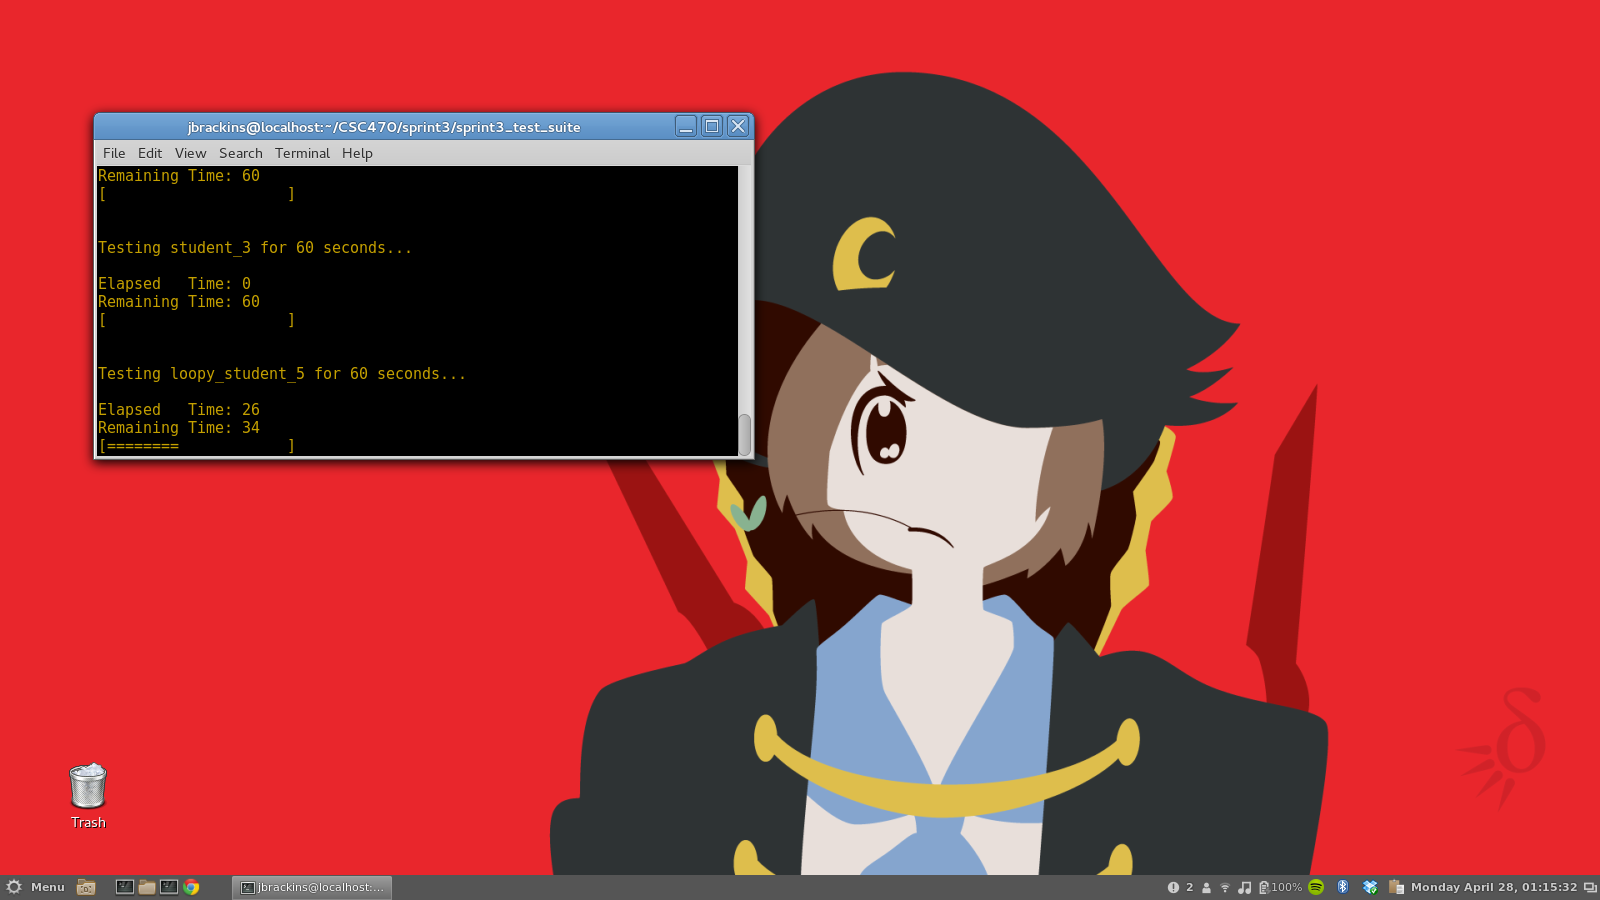
\includegraphics[width=0.6\linewidth]{progbar.png}
				\caption{Progress Bar}
				\label{fig:progbar}
			\end{figure}
			
			We decided to implement a progress bar to display while each students' code is running.
			 This progress bar will show the time that has elapsed, with the start time being
			 "empty" and the end time (maximum time to let a program run) being "full." In
			 Figure 8.3, a program containing an infinite loop has been running for 26 out of a 
			 maximum 60 seconds. When the timer reaches 60 seconds, the process will be killed.
			 
			 			 
		\subsubsection{\large{\color{cyan}Test Case Files}}
			The directory containing the submitted .cpp files must also contain folders of test
			 cases that correspond to the program that will be tested. These must end in .tst.
			 If the user would like there to be a "critical test," or a test that will result in
			 failure if a student's program should fail it, it must contain the extension
			 .crit.test.
		 
		\subsubsection{\large{\color{cyan}Expected Output Files}}
			All expected output files or answer files must end in .ans. They also must have the
			 same name as their corresponding .tst files.
			 
		\subsubsection{\large{\color{cyan}.log Files}}
			The program will create a number of .log files. There will be one in the main
			 directory of the program, and one in the directory for each student. The common
			 summary log file will have grades for all of the students, while the individual
			 log files will have information on which test cases that student may or may not have
			 passed, as well as gcov and gprof information.\\ \ \\We determined that the "golden" 
			 .cpp file should contain all log files so that if the professor or TA desires, they
			 are able to compare the performance of the "golden" .cpp to the performance of the
			 student .cpp files.
			 
			\begin{figure}[h!]
				\centering
				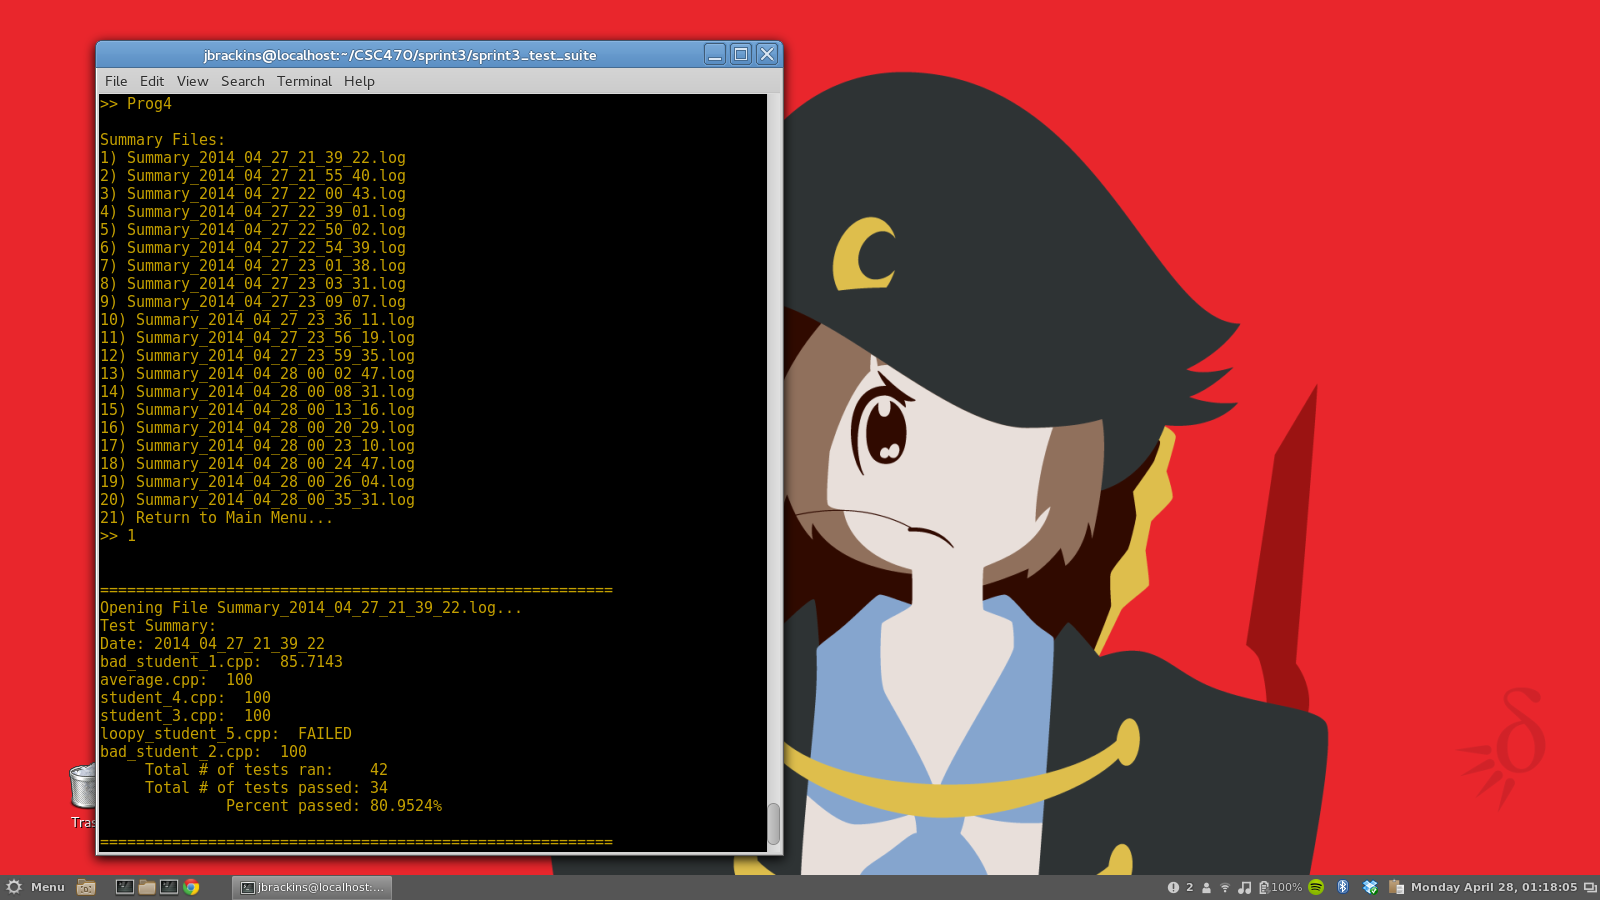
\includegraphics[width=0.6\linewidth]{viewsumm.png}
				\caption{Selecting Summary Files}
				\label{fig:Summary_files}
			\end{figure}
			 
			 
		\subsection{\Large{\color{blue}Installation Guide}}
			To install the program, simply compile it by using the command "make" and run it in 
			 the directory above the student program directories.
			 
		\subsection{\Large{\color{blue}Programmer Manual}}
			The programmer simply needs a text editor and the GNU compiler collection to edit
			 and test the source code.
			 
	\newpage
	
	\section{\LARGE{\color{blue}Class Index}}
		\subsection{\Large{\color{blue}Class List}}
			Not Applicable.
			
	\newpage
	
	\section{\LARGE{\color{blue}Sprint Reports}}
		\subsection{\Large{\color{blue}Sprint Report \# 1}}	
			This sprint lasted from 2/4/14 from 2/19/14. The members of the Whitespace Cowboys
			 setup Github accounts as well as repositories on both personal Linux and Windows
			  machines. Two offical scrum meetings were held, the first of which was to set up
			   Github and the second of which was to assign different members to the writing of
			    sections of documentation and hold a code review. 

			The coding section of the project was officially done on 2/14/14, when the code review
			 was held. The team members made sure the coding and the coding standard were up to
			  requirements, as well as checked the state of the current documentation in the .cpp
			   file. 	 
		 
		\subsection{\Large{\color{blue}Sprint Report \# 2}}	
		 	This particular sprint lasted from 2/21/14 to 3/23/14.  The members of Lounge Against
		 	 The Machine reworked existing code to facilitate multiple programs of execution and a
		 	  new generator system for test and answer file manufacture.  The coding started
		 	   shortly after the beginning of the sprint, but was delayed over spring break for a
		 	    vacation of the Tech Lead.  The project was finished and submitted on 3/23/14 where
		 	     this document was updated with all relevant changes.  All make and execution
		 	      variables were checked before submission.
		 
		\subsection{\Large{\color{blue}Sprint Report \# 3}}
			This sprint lasted from 3/23/14 to 4/28/14. The members of Latex Samurai worked on code
			 provided by Lounge Against the Machine to add more features to the testing suite
			 framework created in sprints 1 and 2. The new features include forking and executing
			 the student .cpp processes, so that they may be killed in the case of an infinite
			 loop, gcov code coverage reports, gprof performance reports, the ability to test
			 CSC150 programs containing a text-based menu loop, and an attractive user interface
			 for our own program.	
		
		
	\newpage
	\addcontentsline{toc}{section}{\LARGE{\color{blue}Acknowledgements}}
	\section*{\LARGE{\color{blue}Acknowledgements}}
		For the help and guidance they have provided throughout the course and the projects, we
		 would like to extend our sincere thanks to Dr. Logar. We have gained valuable knowledge
		 and skills relevant to being a software engineer in industry.\\ \ \\ 
		 We would also like to extend
		 our thanks to Brian Butterfield for making time for our entire class. His presentations
		 provided excellent insight into the workings of a real-world company, and his examples
		 tied in to the course material very well.	
		 
		 
	\newpage
	\addcontentsline{toc}{section}{\LARGE{\color{blue}Supporting Materials}}
	\section*{\LARGE{\color{blue}Supporting Materials}}
		No supporting materials.
		
		
	\newpage
	\addcontentsline{toc}{section}{\LARGE{\color{blue}Industrial Experience}}
	\section*{\LARGE{\color{blue}Industrial Experience}}
		The following pages are the resumes for the members of Latex Samurai.
			\subsection{\Large{\color{blue}Resumes}}	 
		 		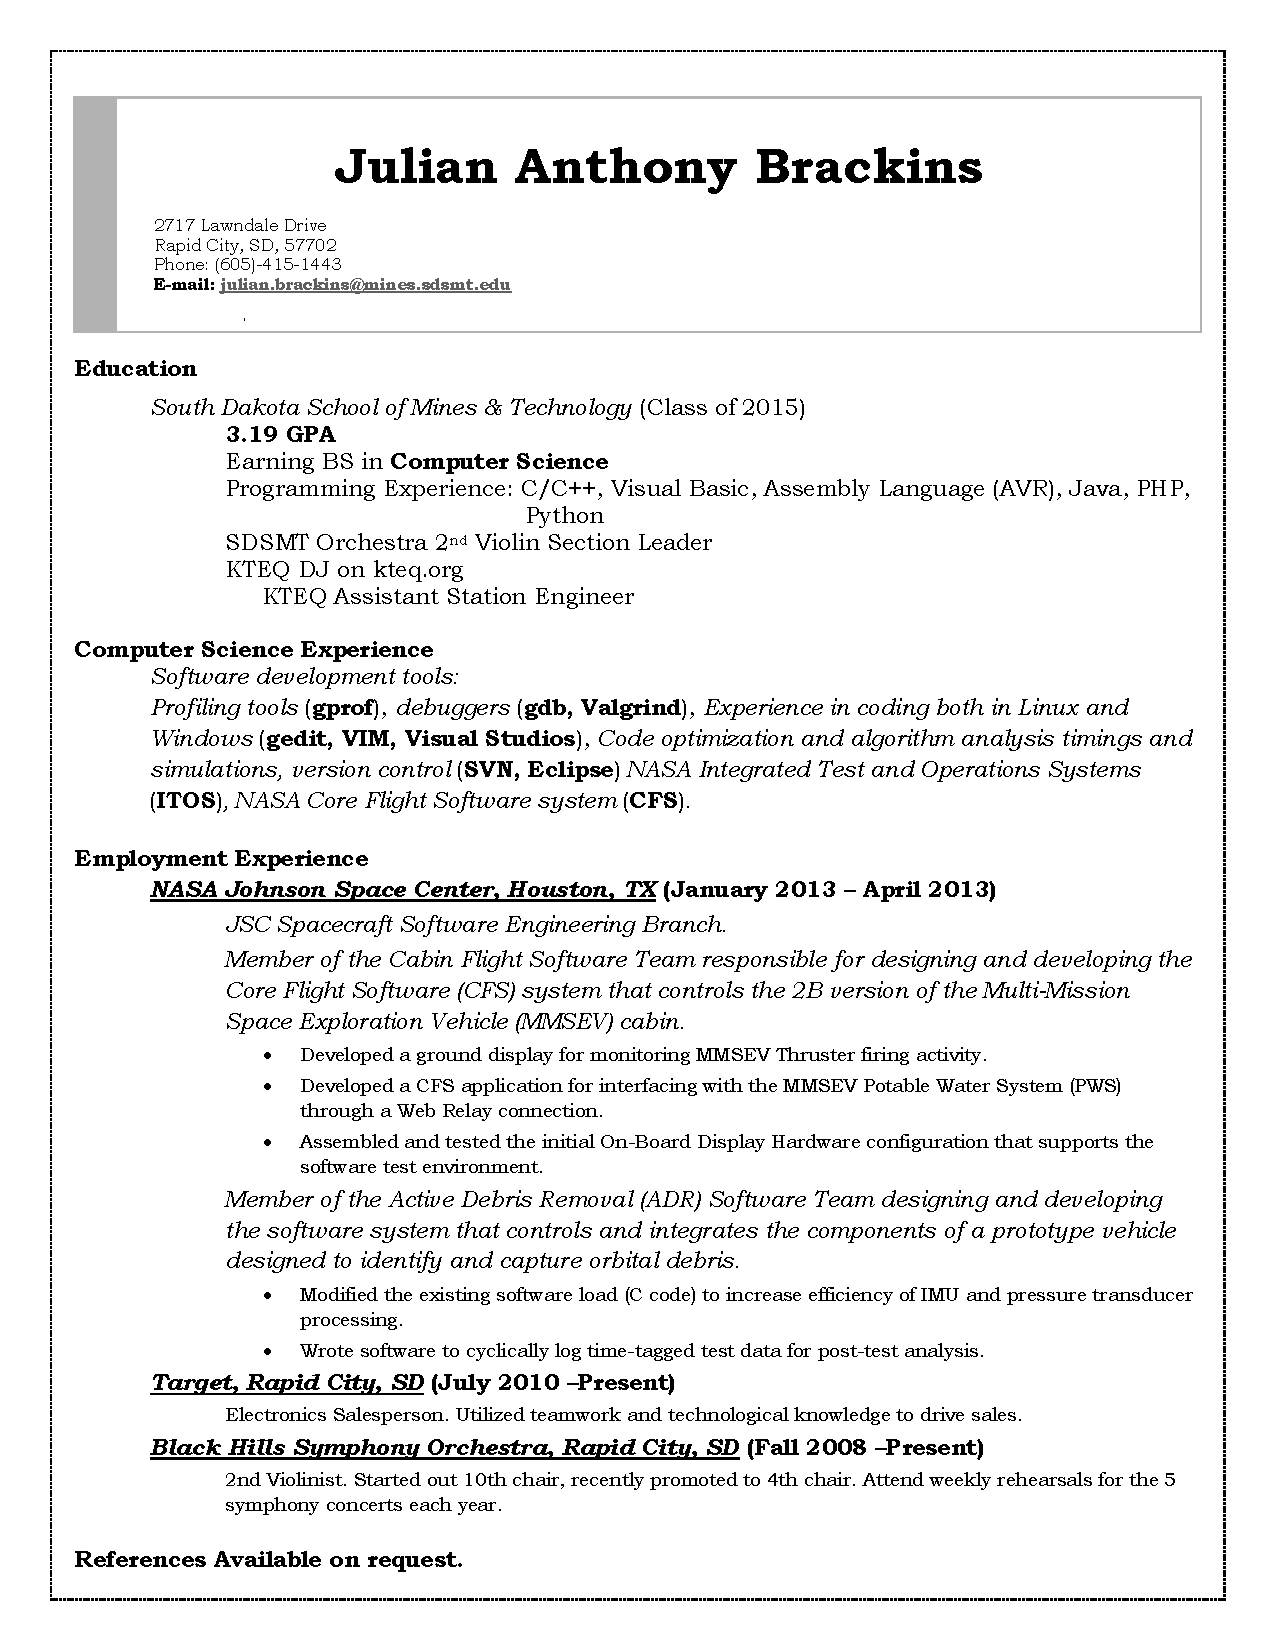
\includepdf[pages={1}]{JB.pdf}
		 		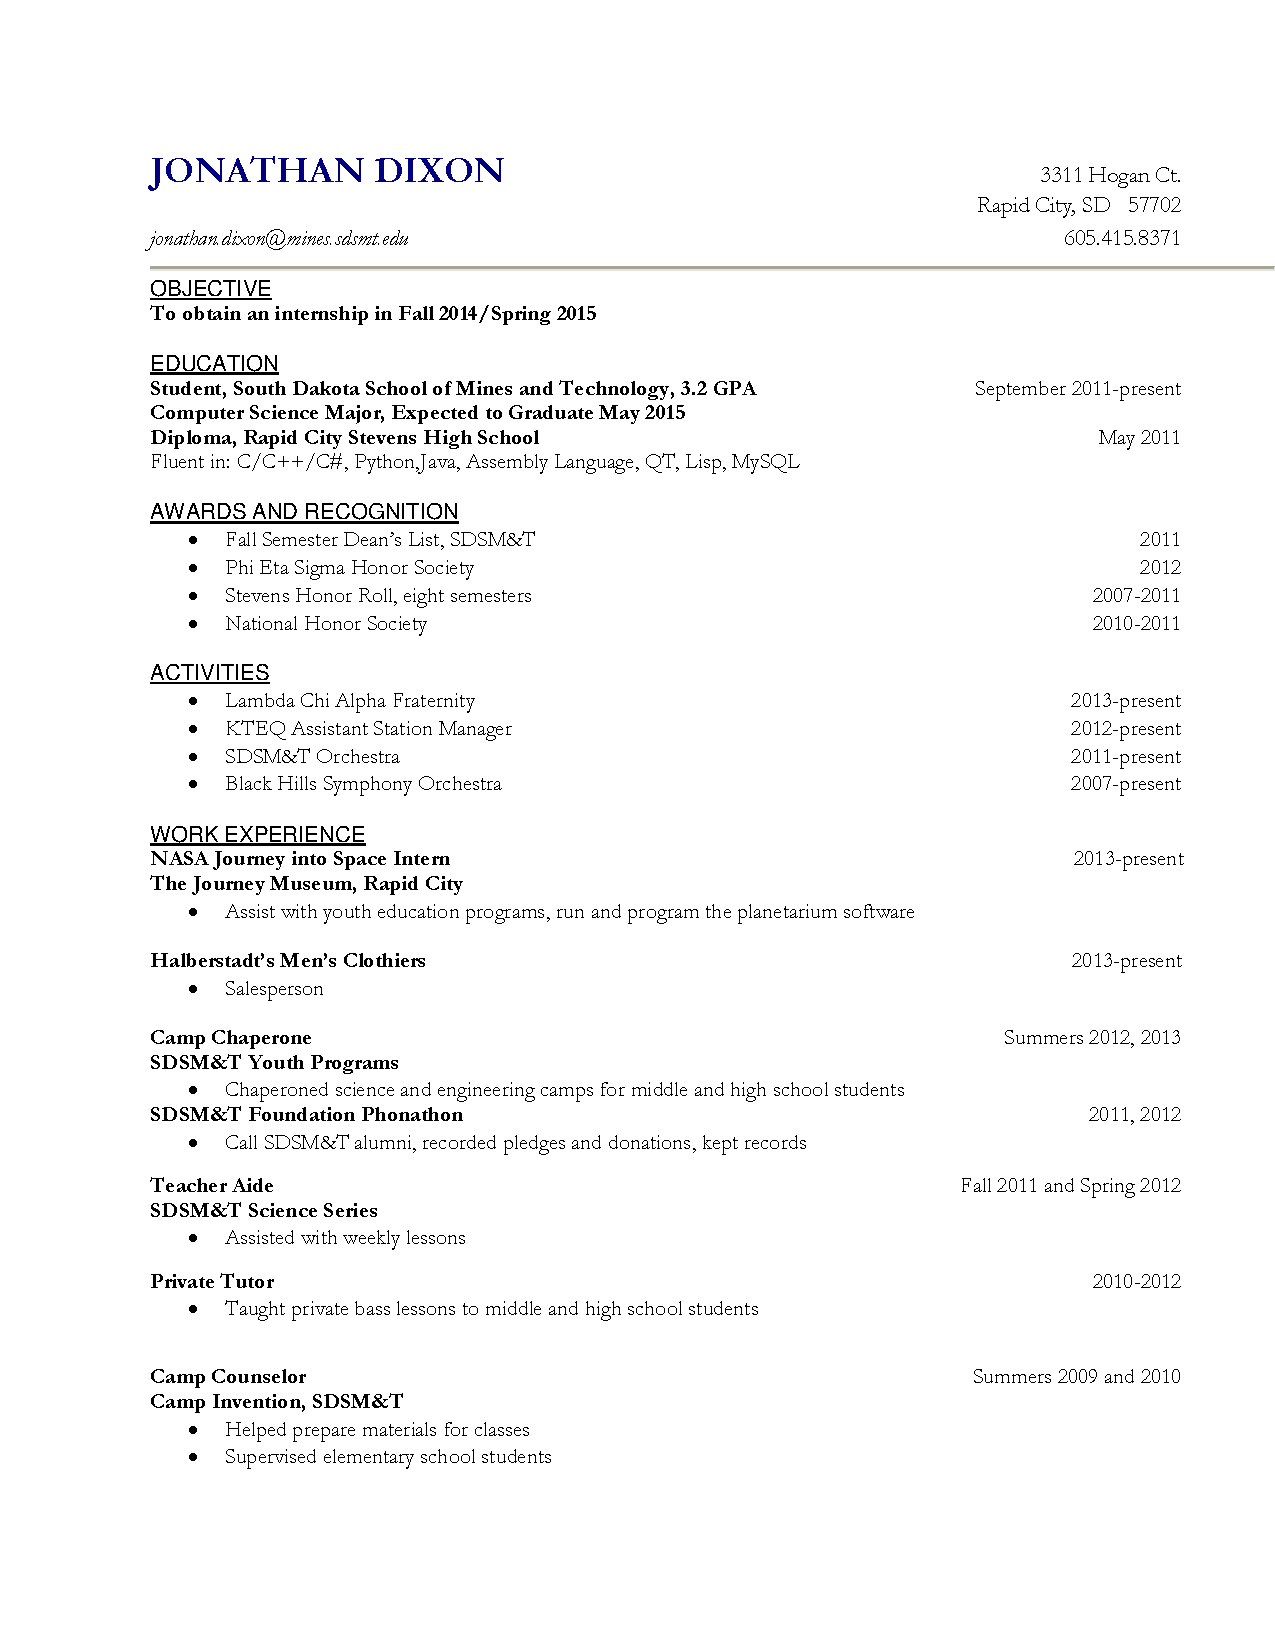
\includepdf[pages={1}]{JD.pdf}
		 		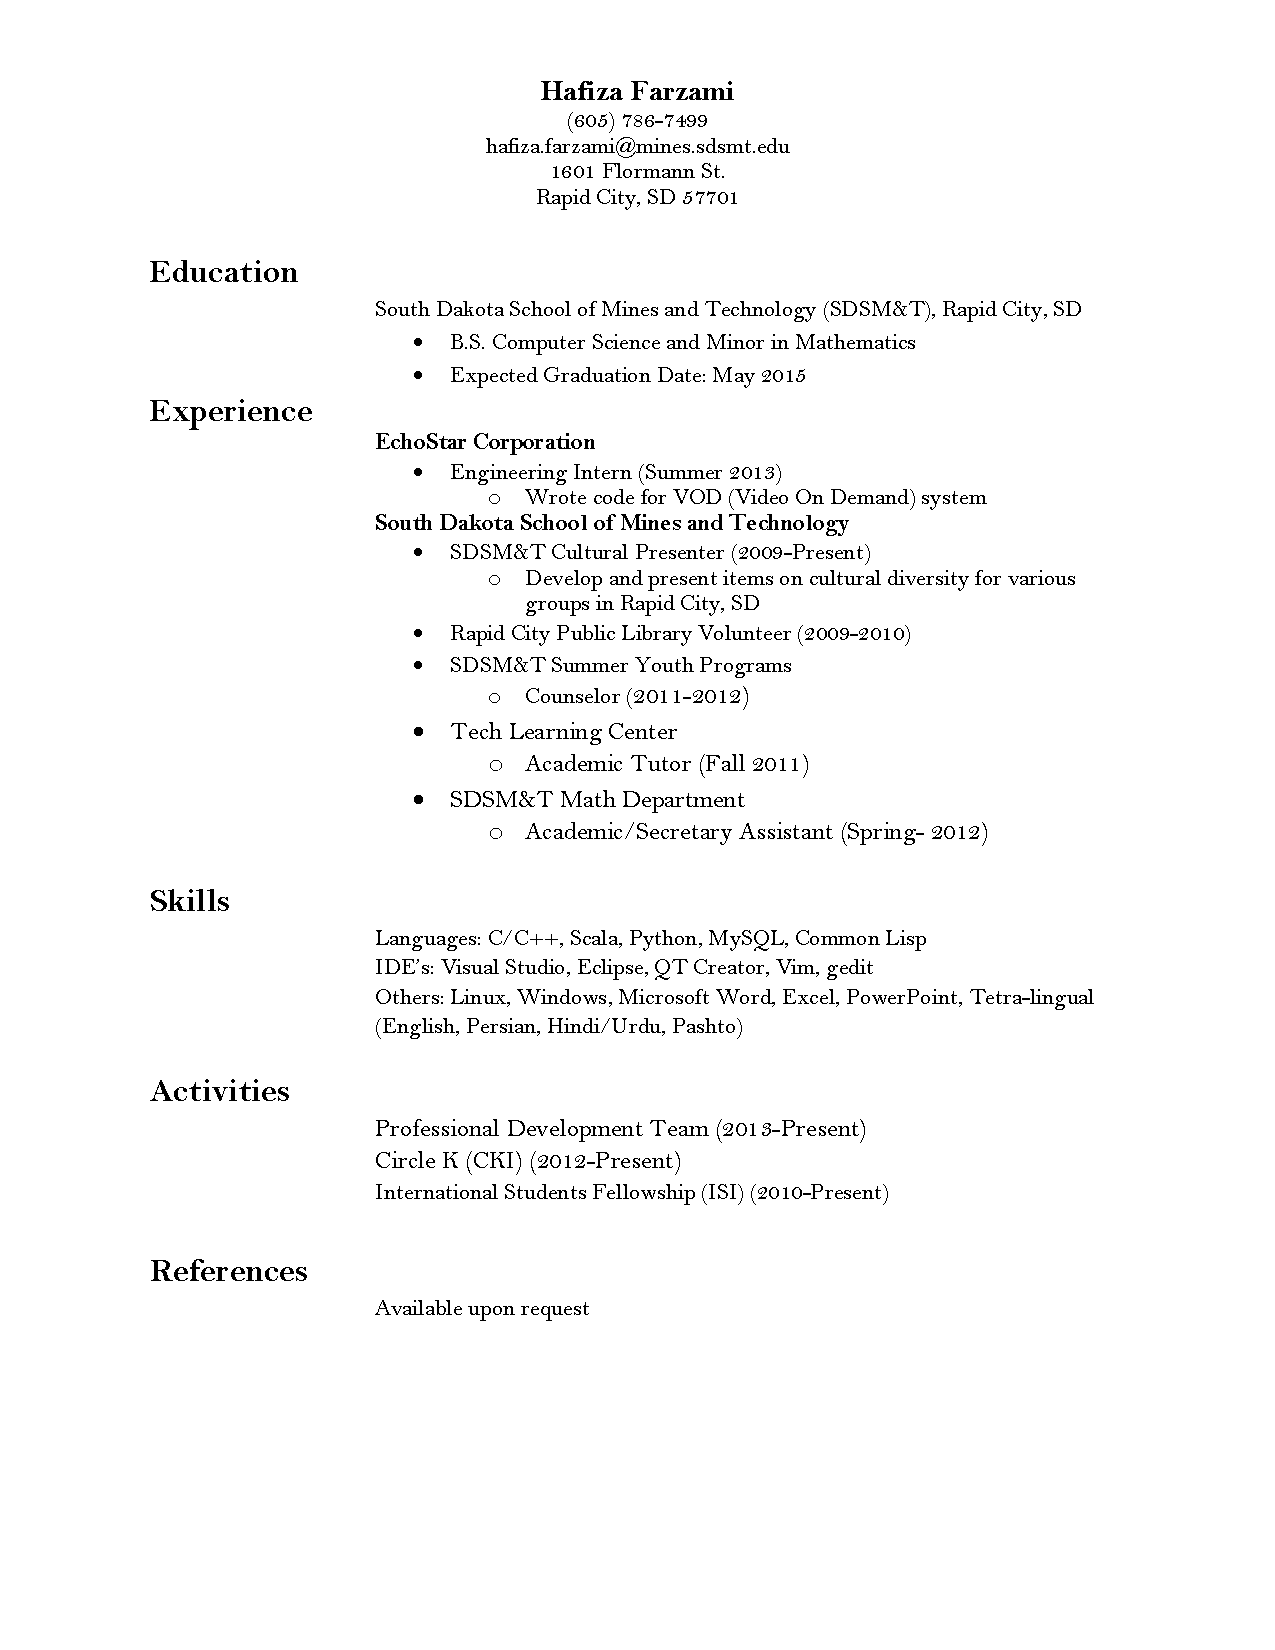
\includepdf[pages={1}]{HF.pdf}
		 		
		 		
	\newpage
	\addcontentsline{toc}{section}{\LARGE{\color{blue}Bibliography}}
	\section*{\LARGE{\color{blue}Bibliography}}	
		No sources cited.	
		 			 
\end{document}